\chapter{Image segmentation}

Image segmentation will be described in this chapter as well as several basic segmentation techniques.
Subsequently level set techniques will be introduced, defined and explained in more detail.
Then level set computation issues will be described along with mentioning of two basic speed-up approaches.
After that level set method relation to image segmentation will be mentioned.
After all some features of the level set computation on streaming architectures will be listed along with comparison to the \mbox{Cell/B.E.} features.

\section{Problem formulation}
Image segmentation is process when pixels of an input image are split into several subsets, segments, based on their characteristics or computed properties, such as colour, intensity, or texture.
The pixels in such segments have similar features and compose an object in the image.

In more formal way it is a function that assign a segment to a pixel:
\begin{equation}
S: S(p) = k
\end{equation}
where $p \in$ pixels of the image and $k \in$ set of segments.

Image segmentation is used in many domains such as medicine (locating organs, tumors, bones, etc.), satellite images classification for maps (location buildings, roads, etc.), machine vision (fingerprint recognition, face, eyes, or other features recognition).
Other example of image processing application can be a simple tool as the well known "magic-stick" tool in popular graphics editing software like Photoshop.

\par
Although there were some attempts to find general-purpose segmentation solution, results were not satisfactory.
So there is not yet a general solution.
Each domain needs extra approach how to perform the segmentation.
Some of them are not even fully automatic so they need assistance of an operator.
They are called semi-autonomous approaches.
These methods need an operator who inputs some region and thus gives a hint to the algorithm.
This is favourite approach in segmentation of structures in medical images like organs, tumors, vessels, etc.
A physician then plays the role of the operator because of his knowledge of images' content.
Some methods are autonomous but need some apriory knowledge of the segmented object properties.

\section{Image segmentation methods overview}

Image segmentation methods can be divided into following basic categories (information based on \cite{wiki}):

\begin{enumerate}

  \item Clustering

  These methods are used to partition an image into $N$ clusters that cover the entire image.
Two main subsets of the methods are bottom-up and top-bottom.
The first one takes each pixel as separate cluster and then iterate joining these initial clusters based on some criterion until there are $N$ clusters.
The second one picks $N$ randomly or heuristic chosen cluster centres.
Then these two steps are repeated until some convergence condition is met e.g. no pixels change clusters: assign pixels to clusters based minimalization of the variance between the pixel and the cluster centre and re-compute the cluster centres by averaging all of the pixels in the cluster.

  \item Histogram-based

  Firstly a histogram is computed from pixels of the image.
Then peaks and valleys in the histogram creates the segments in the image.
Result can be refined by recursively repeating the process.
The recursion is stopped when no more new segments appear.

  \item Edge detection

  These methods segment an image based on its edges.
Therefore core of such methods is an edge-detection algorithm such as Canny, Sobel.

  \item Region growing

  This set of methods are very similar to the flood-fill algorithm.
It takes a set of seed points and a segmented image.
Each seed point is something like pointer to segmented object on the image.
Seed points form an initial set of segments.
Then iteration through the neighbouring pixels of the segments is performed.
In every step of that iteration a neighbour pixels of a segment is compared with the segment i.e. similarity function is calculated.
If the pixel is considered similar enough it is added to the segment.
Method is highly noise-sensitive.
The initial seeds can be misplaced due to the noise.
Therefore there is another algorithm that is seedless.
It starts with a single pixel that is an initial region.
Its location does not significantly influence the final result.
Then the iteration over the neighbouring pixels are taken just as in seeded growing.
If a neighbour is different enough new segment is created.
A threshold value is used as similarity measurement but particular approaches differs in definition of the similarity function.
While one group uses pixel's properties like intensity or colour directly another computes some statistical test from the properties and the candidate pixel is processed according the test is accepted or rejected.

  \item Graph partitioning

This approach converts an image into a graph.
The pixels correspond to the vertices.
There is edge between every pair of the pixels.
Edges are weighted with similarity function of the two connected pixels.
Then a graph algorithm that cuts off edges is run partitioning the graph resp. image.
Popular algorithms of this category are the random walker, minimum mean cut, minimum spanning tree-based algorithm, normalized cut, etc.

  \item Watershed transformation

  The watershed transformation considers the gradient magnitude of an image as a topographic surface.
Pixels having the highest gradient magnitude intensities correspond to watershed lines, which represent the region boundaries.
Water placed on any pixel enclosed by a common watershed line flows downhill to a common local intensity minimum.
Pixels draining to a common minimum form a catch basin, which represents a segment.

  \item Model based segmentation

  The main idea of this method is to describe the segmented object statistically, constructing a probabilistic model that explains the variation of the object shape.
In segmentation phase is the model used to impose constraints as prior.
Searching for such model contains steps like: registration of the training examples to a common pose, probabilistic representation of the variation of the registered samples and statistical correspondence between the model and the image.

  \item Level set

\par
It is a method that uses a mathematical model of the segmented object.
It is represented by a level set function.
Segmentation is performed by deformation of an initial isoline (for 2D case), hyperplane of the level set function, with forces that are computed from the segmented image.

\par
Whole process can be illustrated in very similar way to the flood-filling, see the figure \ref{fg:flooding}.
The initial isoline is deformed with forces that has direction of an isoline normal.
For 2D case the initial isoline can be e.g. a simple circle as a hyperplane of a distance function from a given point.
When it approaches object borders the propagation slows down.
On the object borders the propagation stops because the forces are zero there.

\begin{figure}
    \centering
    
\includegraphics[width=12cm]{data/flooding}
    \caption[Flooding an object]{An initial shape, the circle, grows and floods the object on the background.
In contrast to common flood-fill approach, level set method has several parameters that can e.g. prevent flooding beyond the object borders through small holes.}
    \label{fg:flooding}
\end{figure}

\par
Another illustration uses a landscape with a lake.
Water is always at a constant altitude and the surface of the landscape changes in time.
With the changes of the landscape the shoreline of the lake changes as well.
The landscape represents the level set function and the water surface represent the isoline i.e. $k$-level set.

\par
Advantages of the level set method are lack of special treatment of merging and splitting surfaces necessity, few intuitive parameters, ability of topology changing.
The most suiting advantage for our purpose is ability of performance in all dimension without explicit changes in method because we will perform volume segmentation i.e. 3D case of level set.

\end{enumerate}

\section{Level set}

Level set method as proposed by Osher and Sethian \cite{sethianLS} provides numerical and mathematical mechanisms for surface deformation computation as time varying iso-values of level set function using partial differential equations (PDE).

\subsection{Level set theory}

Information in this and following paragraphs are based on \cite{insightIntoImages} and definitions will be for 2D case.
The level set function is a signed scalar distance function
\begin{equation}
\phi : U_{x,y} \rightarrow \mathbb R,
\end{equation}
where $U \subset R^2$ is the domain of the function.
$\phi$ is called embedding and is implicit representation of the segmented object.
Isoline is then a subset of the level set function values, a hyperplane
\begin{equation}
S = \{\vec{x}\mid \phi(\vec{x}) = k\}
\end{equation}
The symbol $S$ represents a $k$-isoline or $k$-level set of $\phi$.
The variable $k$ can be chosen freely, but in most cases it is zero.
The isoline is then called zero isoline, zero level set or dimension insensitively front (will be used further).

\par
Deformation of the front is then described by an evolution equation.
One approach, dynamic, uses one-parameter family of $\phi$ function i.e. $\phi(\vec{x},t)$ changes over time, $\vec{x}$ remains on the $k$-level set of $\phi$ as it moves and $k$ remains constant.
Resulting equation is
\begin{equation}
\label{deformEq}
\phi(\vec{x}(t),t) = k \Rightarrow \frac{\delta \phi}{\delta t} = - \Delta \phi
\cdot \vec{v}.
\end{equation}
Where $v$ represents movement of a point $x$ on the deforming front i.e. positions in time.
All front movements depend on forces that are based on level set geometry which can be expressed in terms of the differential structure of $\phi$.
So following version of equation \ref{deformEq} link formulated:
\begin{equation}
\frac{\delta\phi}{\delta t} = - \Delta \phi \cdot \vec{v} = - \Delta \phi
\cdot F(\vec{x}, D\phi, D^2\phi, ...),
\end{equation}
where $D^n\phi$ is the set of $n$-order derivatives of $\phi$ evaluated at $\vec{x}$.
The term $F(\vec{x}, D\phi, D^2\phi, ...)$ represents the force that influence the movement of a surface point.
This equation can apply to every values of $k$ i.e. every level set of function $\phi$ and is basic equation of level set method.

\subsection{Level set computation}

Computation of surface deformations has to be discretized which means it is performed on discretized space i.e. grid.
Front propagation is then computed from initial model in cycles representing discrete time steps using this update equation:
\begin{equation}
\label{deformEqApprox}
\phi_{i,j}^{n+1} = \phi_{i,j}^{n} + \Delta t \Delta \phi_{i,j}^{n},
\end{equation}
where the term $\phi_{i,j}^{n}$ is discrete approximation of $\frac{\delta\phi}{\delta t}$ referring to the $n$-th time step at a discrete position $i$,$j$ which has a counter part in continuous domain $\phi(x_i, y_j)$.
$\Delta t \Delta \phi_{i,j}^{n}$ is a finite forward difference term representing approximation of the forces influencing the level set, the update term.
The solution is then succession of steps where new solution is obtained as current solution plus update term.

\par
Discretization of the level set solution brings two problems.
Fist one is need of stable and accurate numeric scheme for solving PDEs.
This is solved by the 'upwind scheme' proposed by Osher and Sethian \cite{sethianLS}.
The second one is high computational complexity caused by conversion problem one dimension higher.
Straightforward implementation via $d$-dimensional array of values, results in both time and storage complexity of $O(n^d)$, where $n$ is the cross sectional resolution and $d$ is the dimension of the image.
In case of pictures with size about $512^3$ voxels the level set computation takes very long time.

\subsection{Speed-up approaches}

\par
Because of computational burden of straightforward level set solving some speed-up approaches has been proposed.
They are useful only when only single level set is computed which is the case of image segmentation.
Then is unnecessary to compute solution for given time step over whole domain but only in those parts that are adjacent to the level set.
Beside the most known and used Narrow Bands and Sparse Fields there is an octree based method proposed by Droske et al. \cite{octree}.

\par
Narrow Band, proposed by Adalsteinsson and Sethian \cite{sethianFastLS}, computes embedding only within narrow band, tube.
Remaining points are set constant to indicate that they are not in the tube.
When level set reach the border of the tube, a new tube has to be calculated based on current level set.
Then new run of computations are performed on this new tube until involving level set reaches tube borders again or the computation is stopped.

\begin{figure}
    \centering
    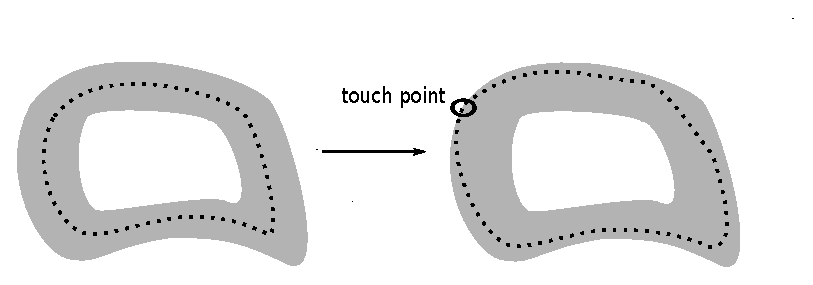
\includegraphics[width=\textwidth]{data/narrowBands}
    \caption[Narrow band computation illustration]{Embedding computation is performed only within narrow band (highlighted in grey). When level set touches (highlighted by the circle) the border or the band, new band has to be computed i.e. reinitialized.}
    \label{fg:narrowBands}
\end{figure}

\par
Sparse Fields method, proposed by Whitaker \cite{sparseFilelds}, introduces a scheme in which updates of an embedding are calculated only on the level set.
This means that it performs exactly the number of calculations that is needed to calculate the next position of the level set.
This is the biggest advantage of the method.

\par
Points that are adjacent to the level set are called active points and they form an active set.
Because active points are adjacent to the level set, their positions must lie within certain range from the level set.
Therefore the values of an embedding in active set positions must lie on certain range, the active range.

\par
When active point value move out from the active range, it is no longer the active point and is removed from the active set.
And vice versa, the point whose value comes into active range is added into active set.
Along the active set there are few layers of points adjacent to the active set organized like peels of an onion, see the figure \ref{fg:sparseFilelds}.

\par
Process of front propagation can be imagined as a tram that lays down tracks before it and picks them up behind.

\begin{figure}
    \centering
    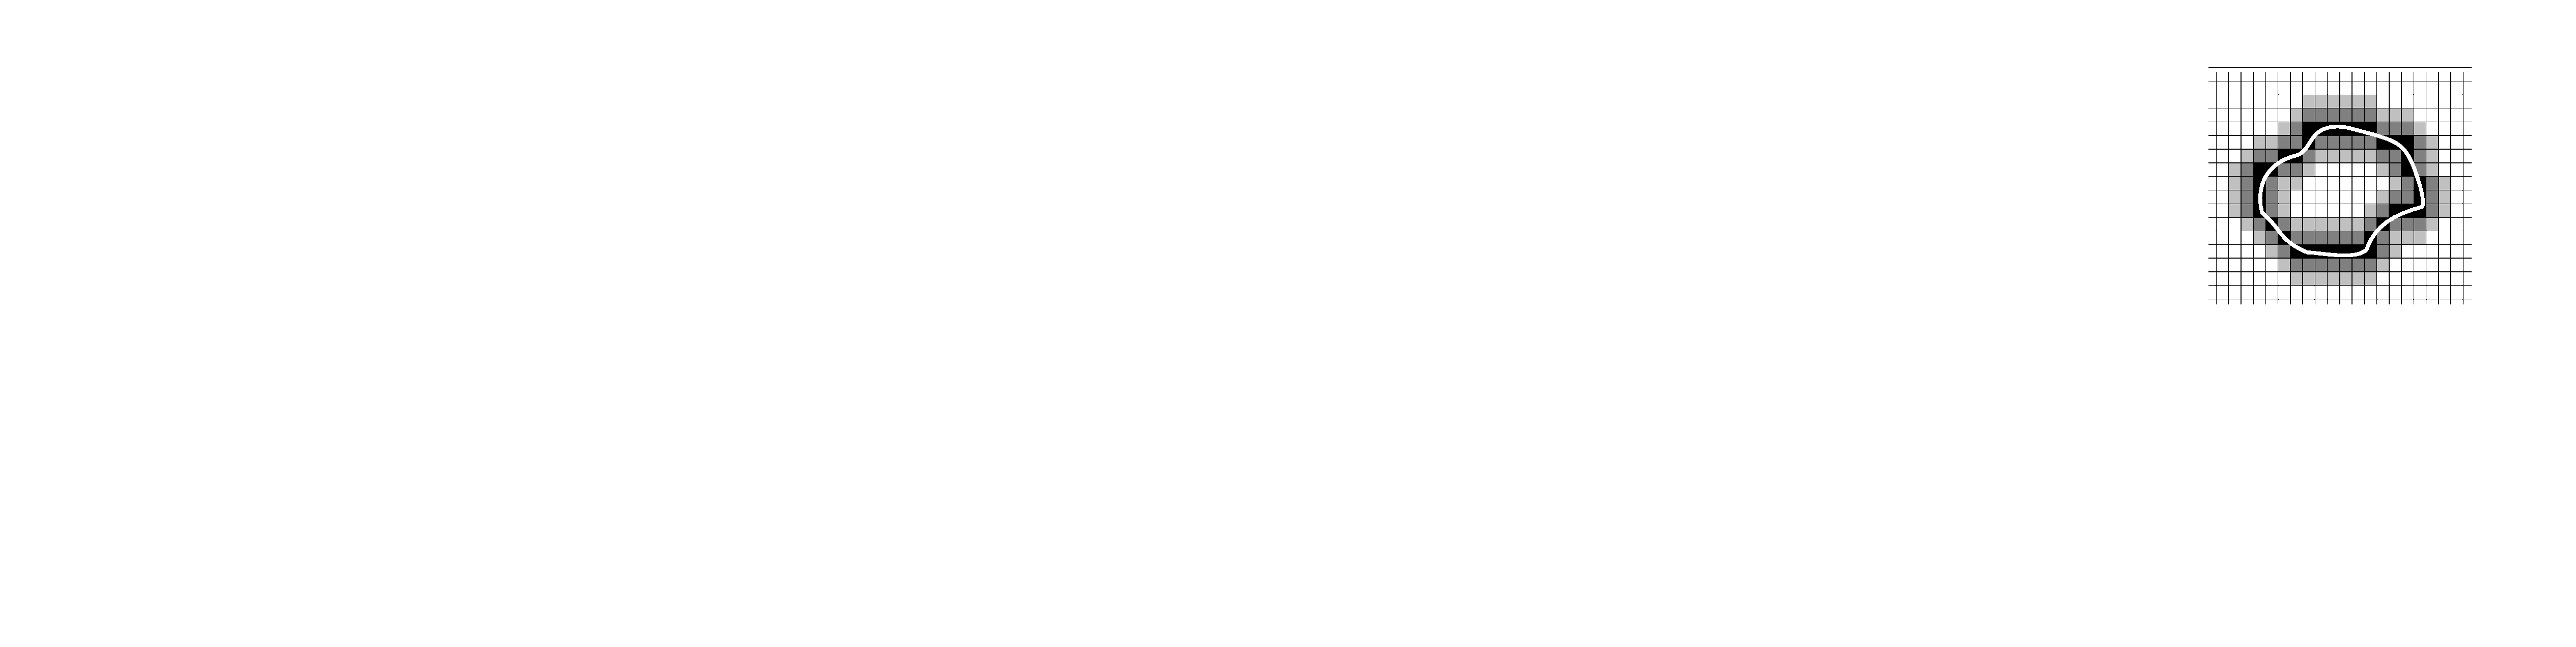
\includegraphics[width=0.9\textwidth]{data/sparsefield}
    \caption[Sparse fields method computation illustration]{Embedding is calculated only at points that are covered by the level set (the white line). Those points (active set) are coloured in black forms the zero layer. Other layers embrace the zero layer from both inner and outer side, formed like onion peels}
    \label{fg:sparseFilelds}
\end{figure}

\par
Algorithm (from \cite{insightIntoImages}):\\
\label{alg:sparseFileld}
\emph{layer, $L_i$} - set of points that are close to the level set. $i$ is order of a layer, negative for inner layers, positive for outer ones. 
Zero is for the active set layer. See the figure\ref{fg:sparseFilelds}\\
\emph{statuslist, $S_{i}$} - list of points within $i$-th layer that are changing status

\par
DO WHILE (stop condition is met):
\par
1) FOREACH (point $\in$ active set, the zero layer (ZL)\\
  a) compute level set geometry $(\vec x)$\\
  b) compute change using the upwind scheme in point $(\vec x)$
\par
2) FOREACH (point $\in$ active set compute new embedding value $\phi_{i,j,k}^{n+1}$, which means computing \ref{deformEqApprox}.\\
Decide if it falls into [-$\frac{1}{2}$,$\frac{1}{2}$] interval.
If $\phi_{i,j,k}^{n+1}$ moved under the interval, put the $(\vec x)$ into lower status list, resp. into higher if $\phi_{i,j,k}^{n+1}$ moved above the interval.
\par
3) Visit points in other layers $L_i$ in order $i=\pm 1,\ldots, \pm N$, and update the grid point values based on the values of the next inner layer $L_{i\pm1}$ by adding resp. subtracting one unit.\\
If more than one $L_{i\pm1}$ neighbour exists then use the neighbour that indicates a level curve closest to that grid point. i.e. use the point with maximal value for the outside layers resp. point with minimal value for the inside ones.
If a grid point in layer $L_i$ has no $L_{i\pm1}$ neighbours, then it gets denoted to the next layer away from the active set, $L_{i\pm1}$.
\par
4) For each status list $S_{\pm1}$, $S_{\pm2}$, $\ldots$, $S_{\pm N}$ do the following:\\
  a) For each element $x_j$ on the status list $S_i$, remove $x_j$ from the list $L_{i\pm1}$ and add it to the $L_{i}$ layer.
Or in the case of $i=\pm (N + 1)$, remove it from all layers.\\
  b) Add all $L_{i\pm1}$ neighbours to the $S_{\pm1}$ list.

\par
The stop condition is specified by maximal count of iterations.
Another stopping criterion is based on a measurement of the front movement.
When the front does not move anymore, calcultation is stopped before maximal count of iterations is reached.

\subsection{Level set image segmentation}

Image segmentation using a level set method is performed based on a speed function that is calculated from the input image and that encourages the model to grow into directions where the segmented object lies.
There is variety of the speed functions.
In this work we used speed function based on a threshold $T_{low}$ and $T_{hi}$ of the intensities if pixels from the input image.
If a pixel has intensity value that is within the threshold interval the level set model grows, see the figure \ref{fg:speedFunction}.
Otherwise it contracts as fast as the pixel has value further from the interval.
The function $D$ is defined as:
\begin{equation}
\label{eq:speedFunction}
D(\vec{x}) =
\begin{cases}
V(\vec{x}) - T_{low} & \text{if $V(\vec{x}) < T_{mid}$}\\
T_{hi} - V(\vec{x}) & \text{if $V(\vec{x}) > T_{mid}$}\\
\end{cases}
\end{equation}
where $V(\vec{x})$ is pixel value in point $\vec{x}$ and $T_{mid}$ is the middle of the thresholding interval.

\begin{figure}
    \centering
    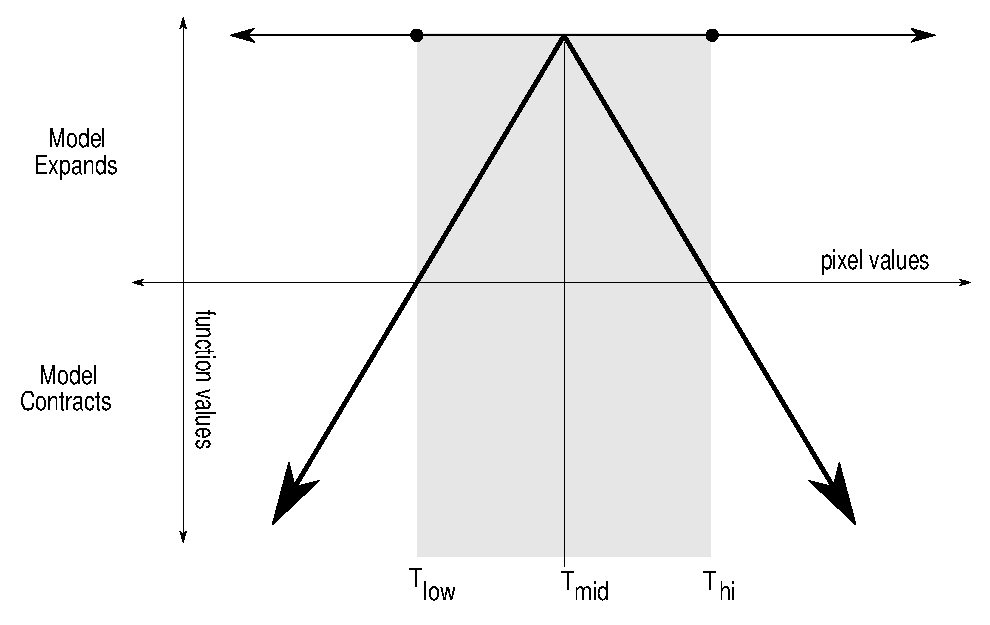
\includegraphics[width=0.9\textwidth]{data/speedFunction}
    \caption[Graph of thresholding based speed function]
    {
      Gray rectangle encloses interval where the speed function is positive, i.e. the model expands.
      The fastest expansion is in the $T_{mid}$ point
    }
    \label{fg:speedFunction}
\end{figure}

\par
This is quite natural definition of what we need from the process i.e. grow as fast as possible where the segmented object lies and contract otherwise.

The update term from equation \ref{deformEqApprox} can be rewritten into following form that consist of few terms:
\begin{equation}
\phi_t = \alpha |\bigtriangledown \phi| H + \beta
\bigtriangledown|\bigtriangledown I|\cdot \bigtriangledown \phi +
\gamma|\bigtriangledown \phi|D
\end{equation}
where $|\bigtriangledown \phi|D$ represents speed function term, $\bigtriangledown|\bigtriangledown I|$ is edge term that is and $|\bigtriangledown \phi| H$ represent curvature term. $\alpha$, $\beta$ and $\gamma$ are weights of particular terms.

Edge term is computed from second order derivatives just like Canny and Marr-Hildreth algorithms for edge detection.
It shall to push level set towards edges, i.e. border of segmented object.

Curvature forces the resulting level set model to have less surface area and thus protect negative effects like leaking into unwanted places shown in the figure \ref{fg:leaking}.
Note: if $\alpha$ = $\beta$ = 0, the result is the same as flood-fill method result because there is only the speed term taking place in the calculations.

\begin{figure}
    \centering
    \includegraphics[width=0.3\textwidth]{data/png/leaking1}
    \includegraphics[width=0.3\textwidth]{data/png/leaking2}
    \includegraphics[width=0.3\textwidth]{data/png/leaking3}
    \caption[Leaking]{Illustration of leaking artefacts.
    Initial level set - circle (left).
    Without curvature forces, segmentation leaks into unwanted places (center).
    Segmentation with curvature forces (right).
}
    \label{fg:leaking}
\end{figure}

We omitted the edge term so there are only two parameters in our method.
Tuning of the term weights has to be performed in order to have the best results.

\subsection{Level set methods on streaming architectures}

\par
There were some attempts for porting level set method onto special stream device.
There are some obstacles due to streaming architecture that has to be overcomed to efficiently solve the problem.
Firstly the streams of data must be large, contiguous blocks in order to take advantage of streaming architecture.
Thus the points in discrete grid near the level-set surface must be packed into data blocks that can be further processed by streaming processors.
Another difficulty is that the level set moves with each time step, and thus the packed representation must be quickly adapted.

\par
For example Cates at al. \cite{GIST} or Lefohn at al. \cite{lefonhGPUSolver} ported level set segmentation method to GPU.
GPU is a streaming architecture with many, nowadays hundreds, of streaming cores.
They run short programs called shaders.
In porting to GPU architecture a texture memory is used to store input data in a large continuous block.
Actual computation is then managed by vertices that flow into the shader and play a role of pointers to the texture memory.
This is some kind of trick because the texture memory is not addressed directly by address number like in single dimension continuous address space in common processors but instead by a 2D coordinate vector.
Because vertices comes as 3D points, virtual memory system that map 3D vertices to 2D texture coordinates has to be created.
Such system proposed Lefonh at al. \cite{lefonhGPUSolver}. See the figure \ref{fg:virtual memory on GPU}.

\par
Another workaround has to be performed when computed data is transferred back to the CPU.
This direction is much slower than the CPU to GPU direction and thus the results has to be somehow packed.
Lefonh at al. \cite{lefonhGPUSolver} describes this packaging as well.
There are although some advantages.
One is the high count of the processors and extreme fast dedicated memory so the results can be impressive.
Another is that the calculation can be directly visualized by the GPU.

\begin{figure}
    \centering
    \includegraphics[width=\textwidth]{data/png/gpuVirtMemory}
    \caption[GPU virtual memory]{Illustration of virtual memory system (taken from \cite{lefonhGPUSolver}). 3D space level set domain (that incoming vertices come from) is mapped via page table to 2D texture coordinate system.}
    \label{fg:virtual memory on GPU}
\end{figure}

\par
Although the \mbox{Cell/B.E.} has some parts of the approach in common with GPU it need not to overcome the GPU obstacles.
For instance no virtual memory system need to be implemented because the SPE has its own flat address space by default.
Also the result packing for sending back to CPU is not necessary because transmission of data from and to SPE has the same speed and can be performed directly.
All these \mbox{Cell/B.E.} processor features could result easier and more straightforward process of porting of level set method.
But speed of the \mbox{Cell/B.E.} result will not probably exceed the GPU solution speed.
